\section[Представление геометрической информации в различных видах ПО]{Представление геометрической информации\\ в различных видах ПО}\label{sec:geoDifferentReprs}

% ================================================================================================================
%   ____    _    ____                                      _              
%  / ___|  / \  |  _ \      __ _  ___  ___  _ __ ___   ___| |_ _ __ _   _ 
% | |     / _ \ | | | |    / _` |/ _ \/ _ \| '_ ` _ \ / _ \ __| '__| | | |
% | |___ / ___ \| |_| |   | (_| |  __/ (_) | | | | | |  __/ |_| |  | |_| |
%  \____/_/   \_\____/     \__, |\___|\___/|_| |_| |_|\___|\__|_|   \__, |
%                          |___/                                    |___/ 
% ================================================================================================================

\subsection{Граничное представление BREP}\label{sec:geoCAD}

Граничное представление (Boundary representation, BREP) --- наиболее распространённый способ точного описания геометрии в ЭВМ, используемый геометрическими ядрами всех современных систем автоматизированного проектирования (САПР).
% Похоже, это первое явление САПР и CATIA народу в тексте (не во всяких списках типа цели, новизна и проч.)
Во многих физических лабораториях, включая CERN, GSI и ОИЯИ, в качестве основной САПР используется система CATIA~v5 (Computer-Aided Three-dimensional Interactive Application), разрабатываемая французской фирмой Dassault Systemes.

\textbf{Далее представление геометрической информации в САПР мы будем называть просто BREP, хотя строго говоря это не совсем верно.}

% Ссылка на Голованова должна появиться где-то
% \todo Утвердить, что тут, а не где-то в другом месте
Геометрическое моделирование в САПР и граничное представление достаточно подробно описаны в работе~\cite{Golovanov}.

В BREP есть два типа понятий --- геометрические (<<точка>>, <<кривая>>, <<поверхность>>) и топологические (<<вершина>>, <<ребро>>, <<грань>>). <<Точка>> --- это тройка координат в некоторой системе координат. <<Кривая>> --- это уравнение, задающее множество точек, принадлежащих данной кривой. Кривую удобно описать с помощью параметрического уравнения от одной переменной. <<Поверхность>> --- это уравнение, задающее множество точек, принадлежащих данной поверхности. Соответственно, поверхность удобно описать с помощью параметрического уравнения от двух переменных. Топологические сущности задаются на базе геометрических. <<Вершина>> лежит в некоторой геометрической точке. <<Ребро>> лежит на некоторой геометрической кривой и ограничено двумя вершинами. Очевидно, что эти вершины должны принадлежать кривой, то есть и соответствующие геометрические точки должны принадлежать кривой. <<Грань>> лежит на некоторой поверхности и ограничена замкнутым циклом из рёбер. Также очевидно, что эти рёбра должны принадлежать поверхности, как и кривые, на которых они лежат, как и вершины и точки, ограничивающие эти рёбра. Замкнутая оболочка из граней с указанием внешних сторон этих граней ограничивает некоторую область пространства, называемую <<телом>>.

В памяти ЭВМ или обменном файле создаётся древовидная структура. Терминальными вершинами этого дерева чаще всего являются геометрические точки, представляющие собой тройки чисел с плавающей точкой. Далее вверх по дереву, имеются узлы типа вершина со ссылками на геометрические точки. Ребро также представляется в виде узла дерева, от которого идёт ссылка на геометрическую сущность, описывающую уравнение кривой, на которой это ребро построено, и ссылки на вершины, ограничивающие это ребро.

В соответствии с BREP параллелепипед (которому эквивалентен примитив box в CSG, см. секцию~\ref{sec:secGeoCSG}) задаётся следующим образом (\figref{fig:BREPbox1} и \figref{fig:BREPbox2}). На этих рисунках дерево представленно упрощённо. Имеется 8 вершин, каждое из 12 рёбер ограничено двумя из этих восьми вершин. Описание вершин не дублируется, на одну и у же сущность может быть множество ссылок. Аналогичным образом каждая из 6 граней ограничена прямоугольником --- циклом из четырёх рёбер, поэтому от каждой сущности типа грань идёт 4 ссылки на рёбра. Тело представляется как замнутая оболочка из поверхностей, поэтому от сущности типа solid идут ссылки на 6 граней. Фактически, помимо представленной на рисунках структуры, имеется ещё довольно-таки много дополнительной информации, без которой корректное и однозначение описание было бы невозможным, например, направления рёбер, направления обхода в цикле из рёбер, направления нормалей граней, уравнения кривых и поверхностей (в данном примере лишь неявно, т.к. используются базовые прямые линии и плоскости), и т.д.

\begin{figure}[H]
\centering
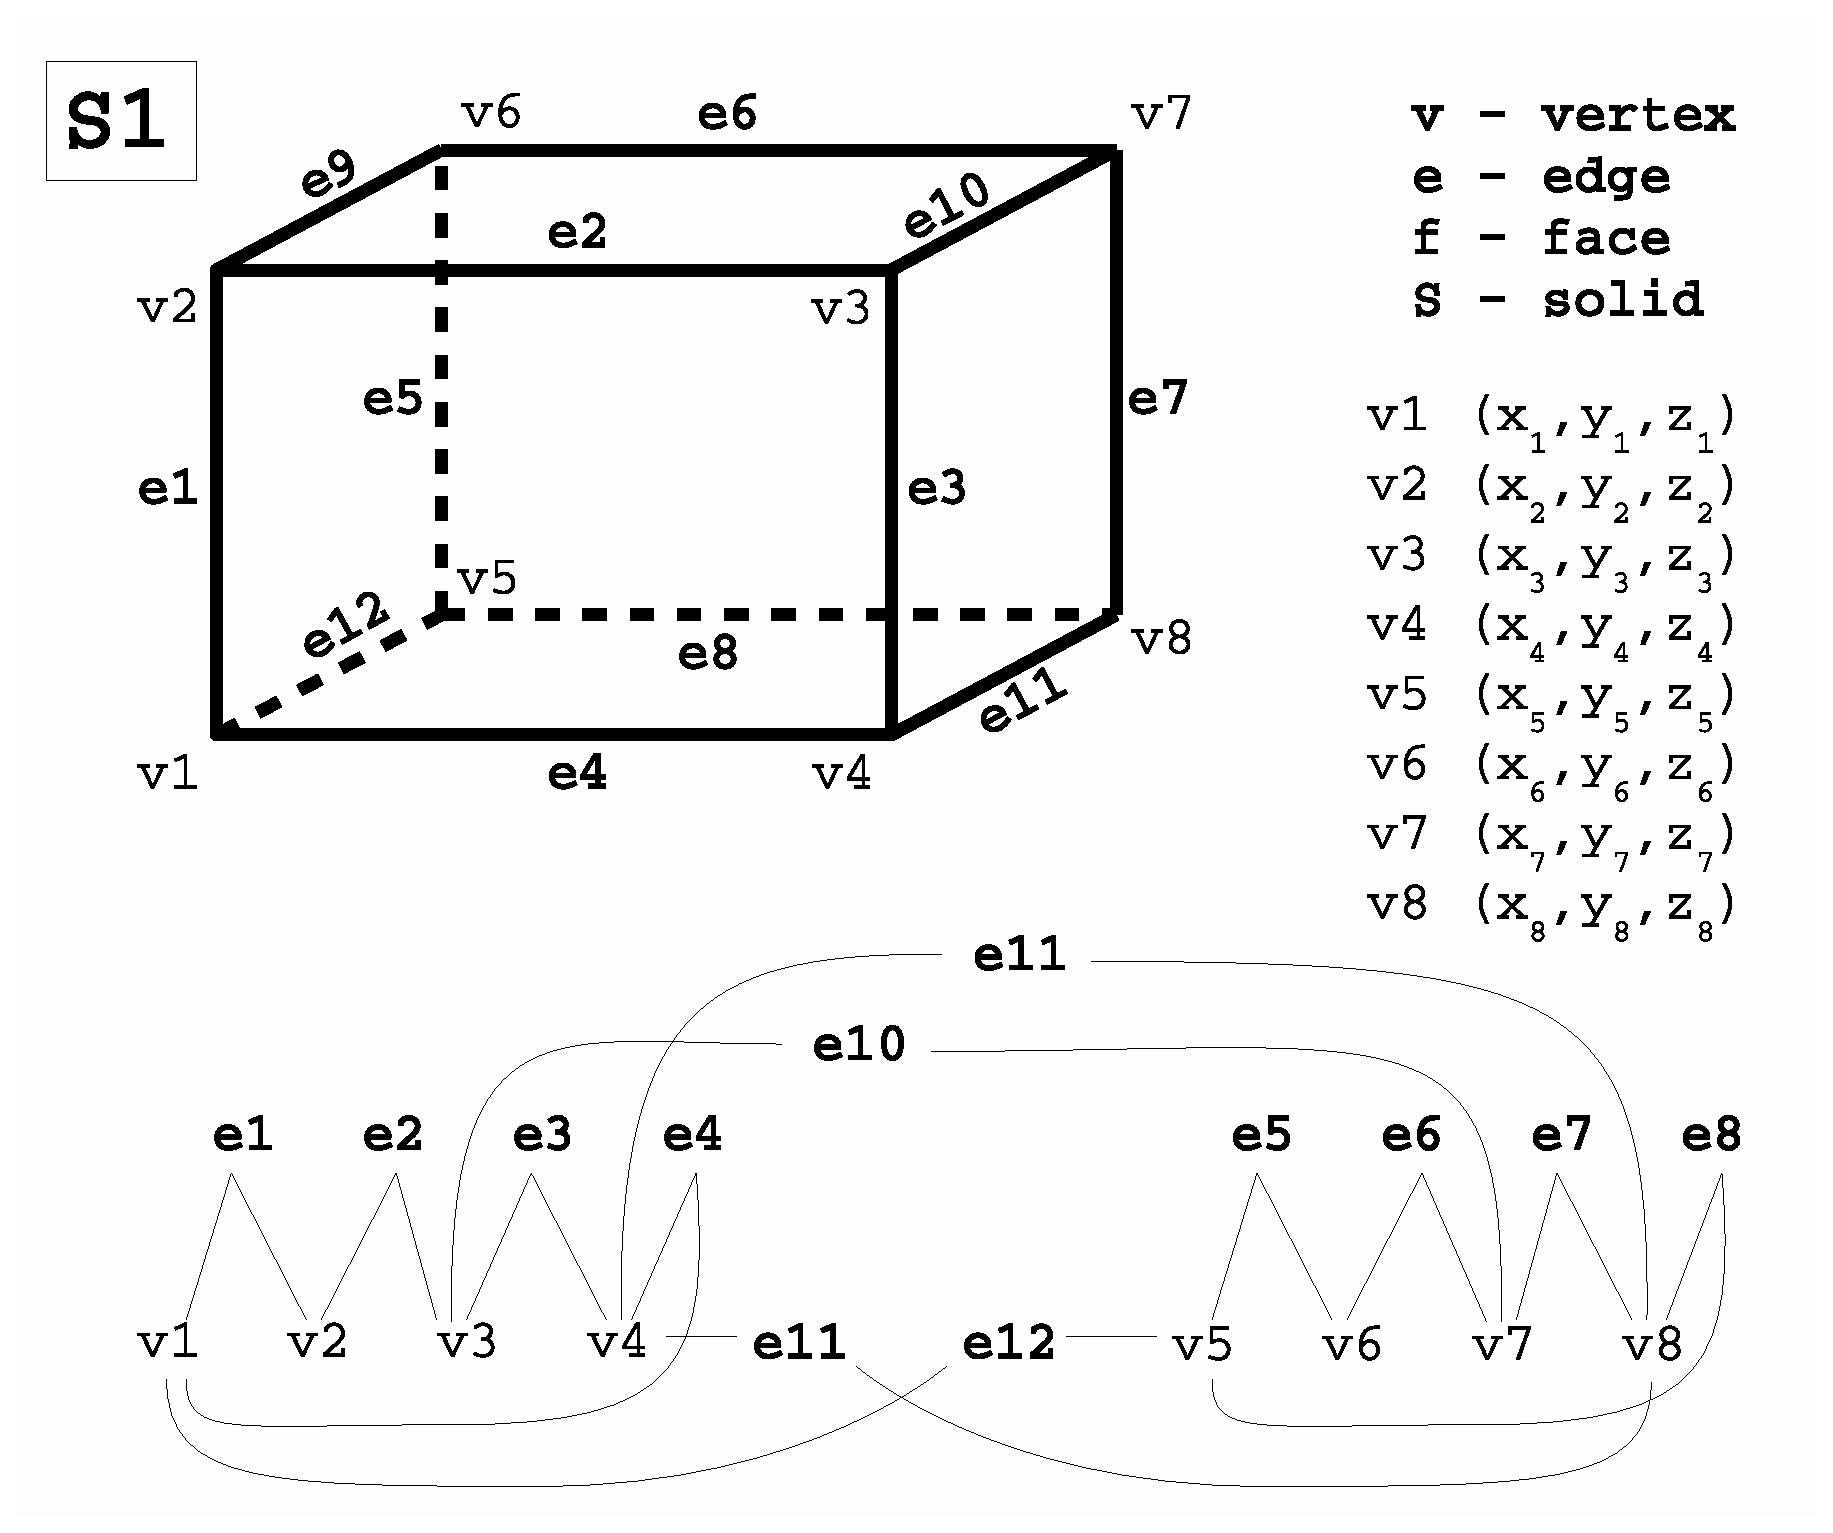
\includegraphics[width=0.7\textwidth]{pictures/BREPbox1.eps}
\caption{Описание вершин и рёбер примитива box методами BREP.}
\label{fig:BREPbox1}
\end{figure}

\begin{figure}[H]
\centering
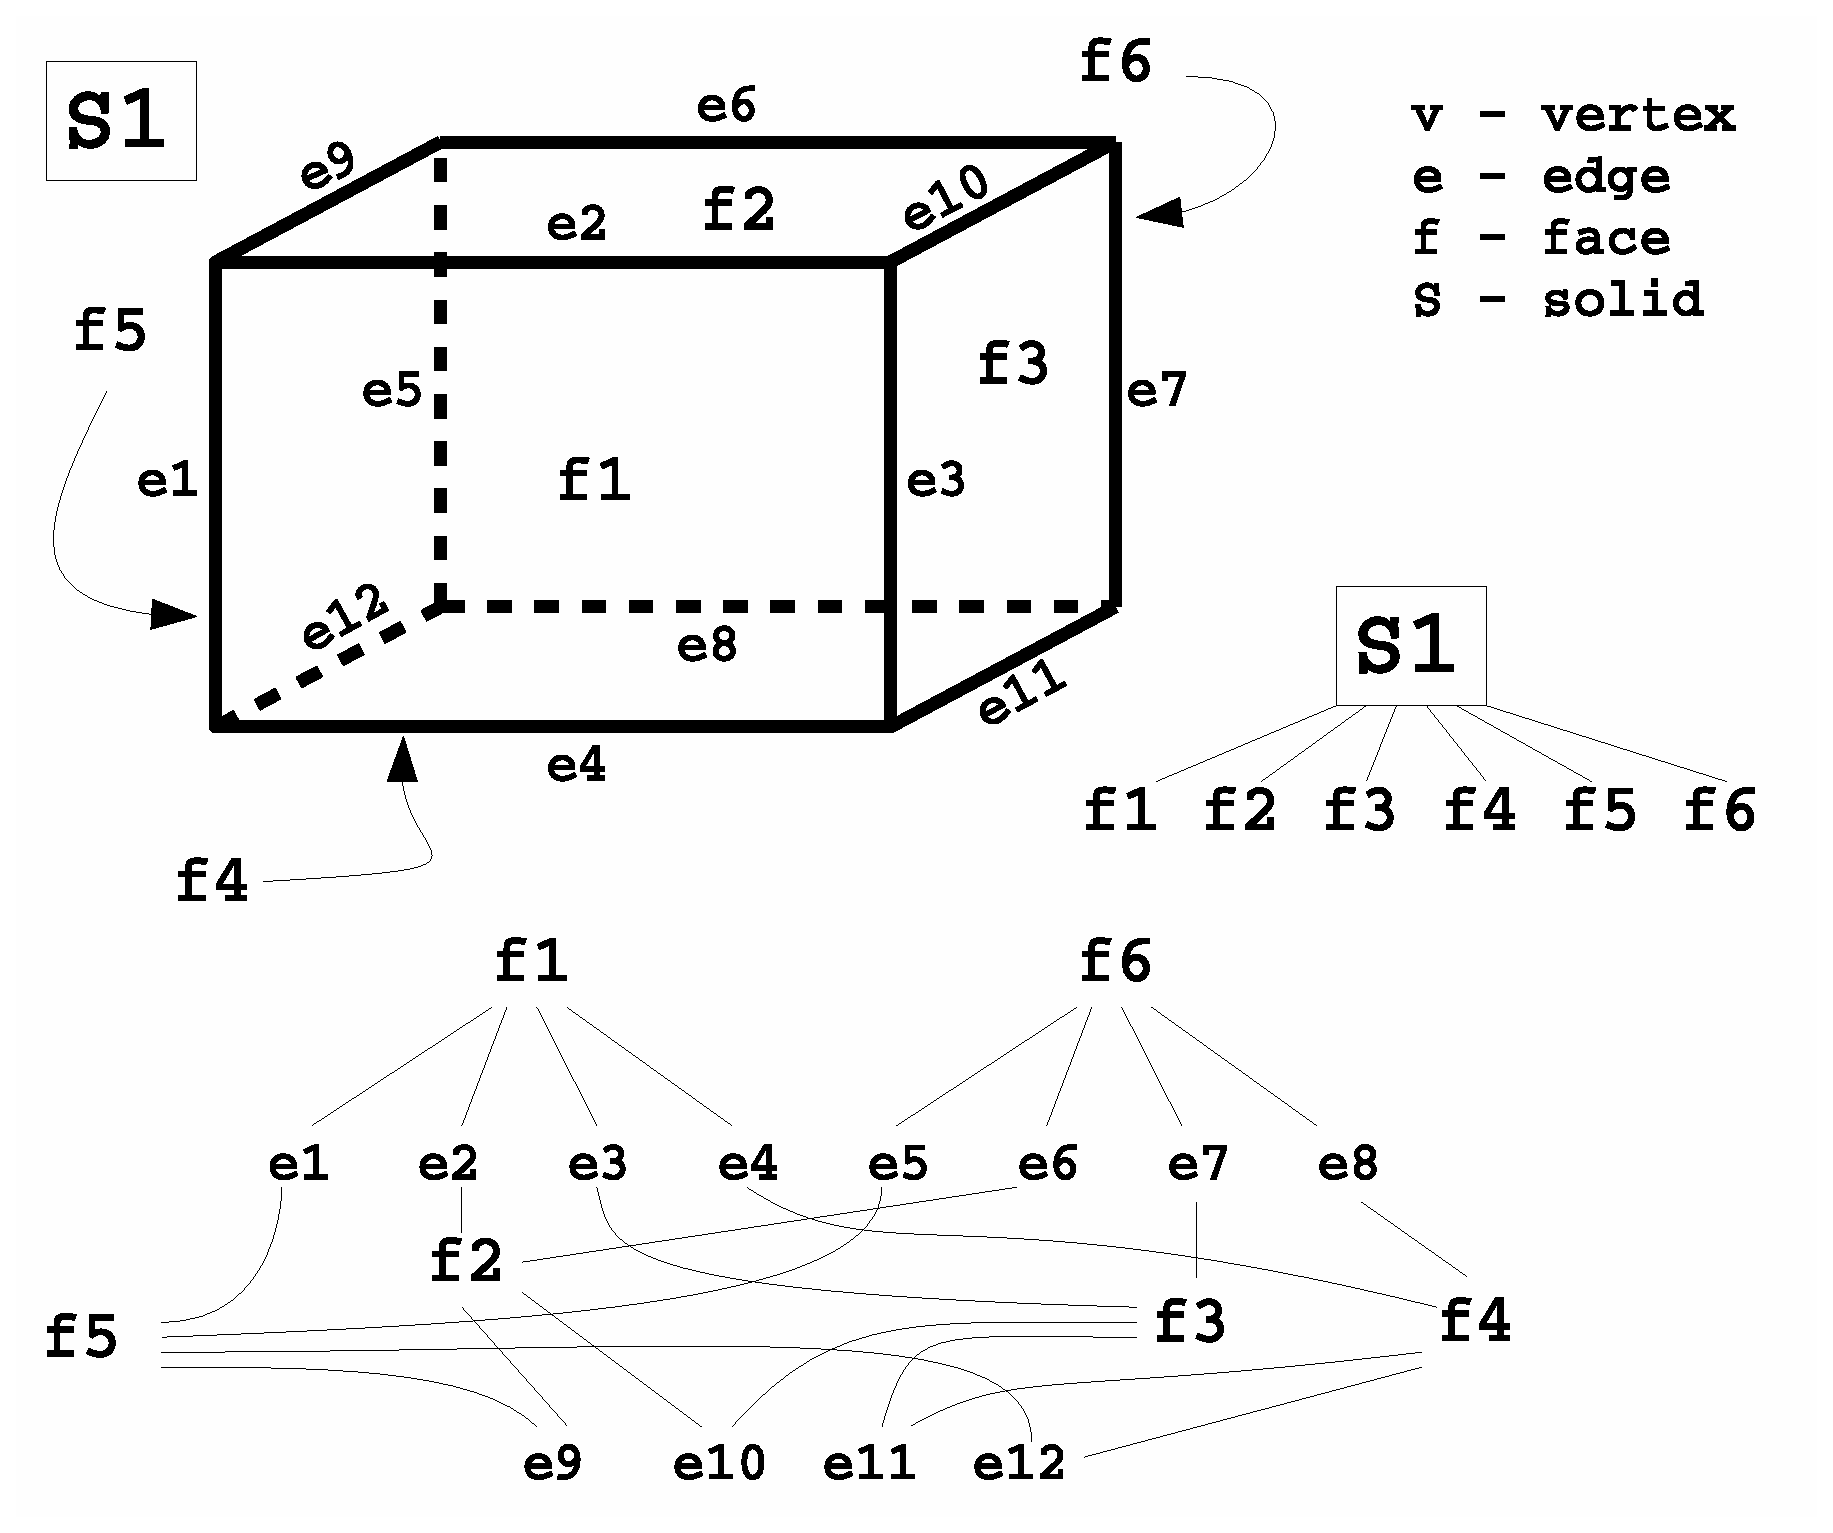
\includegraphics[width=0.7\textwidth]{pictures/BREPbox2.eps}
\caption{Описание граней и тела примитива box методами BREP.}
\label{fig:BREPbox2}
\end{figure}

%Подходы геометрического моделирования, принятые в САПР, обеспечивают максимально эффективную работу как ЭВМ, так и инженеров, в частности за счёт того, что эти подходы интуитивно понятны человеку.

Стоит, однако, отметить, что человек, создающий геометрическую модель в САПР, хотя и может выполнять построения в соответствии с базовыми принципами BREP, чаще всего применяет интуитивно понятные формообразования. Из последовательности этих формообразований система точно формирует BREP модель в памяти ЭВМ, которая также необходима для получения триангулированной геометрии для визуализации на дисплее ЭВМ~(\ref{sec:secGeoPoly}). Есть 4 базовых формообразования и 4 им обратных (с вычитанием) --- <<выдавливание>>, <<вращение>>, <<протягивание>> и <<тело по сечениям>>. Многие другие формообразования, такие как фаски и скругления, разрезы, отверстия, внутри на самом деле являются лишь вариациями перечисленных. Последовательность формообразований, выполненных пользователем для получения итоговой формы, сохраняется в виде дерева построения модели, напоминающего историю построения, но позволяющего навигацию и редактирование. Дерево часто доступно пользователю в основном рабочем окне интерфейса САПР. Однако бывают случаи, когда история построения теряется, например при передаче модели из одной САПР в другую. Таким образом, в результате работы инженера получается модель, описанная с помощью BREP, и во многих случаях имеющая также и дерево построения.

% \todo Пояснить, почему речь о CATIA.
% Ввёл чуть выше - в начале главы.

В инженерной практике принято проектировать и соответственно строить 3d-модели, объединяя в сборки детали и другие сборки. Отсюда вытекает, что во многих САПР, в том числе в CATIA~v5, существуют стандартные объекты, обозначающие детали и сборки. Например в САПР CATIA~v5 существует отдельный тип документа CATPart для детали и отдельный тип документа CATProduct для сборки. Внутри документа типа CATPart есть минимальный набор обязательных элементов --- 3 стандартные взаимноперпендикулярные плоскости в начале системы координат детали и главное тело детали, по умолчанию называемое PartBody. В документе типа CATProduct присутствует возможность добавлять в качестве дочерних компонентов либо документы CATPart либо другие документы CATProduct. В~\ref{sec:secBuilder} описывается, как соотносятся перечисленные сущности CATIA~v5 с понятиями геометрической подсистемы GEANT/ROOT.

Во многих САПР, в том числе и CATIA~v5 присутствует возможность так называемого контекстного редактирования компонентов. Это означает, что пользователь во время работы над сборкой в документе типа CATProduct, имеющей в качестве дочерних компонентов детали в файлах типа CATPart, может также редактировать эти детали, не переключая активный документ. Эта возможность широко используется в ``CATIA-GDML geometry builder'' --- большая часть работы выполняется в контексте единственного продукта, что с точки зрения пользователя аналогично работе над всей экспериментальной установкой.

%\todo
%Описать только нормальное применение BREP, то есть для замкнутых солидов.
BREP разрабатывался как наиболее общий метод представления геометрии в ЭВМ и не ограничивается описанием твёрдых тел. Отдельные поверхности, например, также являются корректными сущностями.

%Более того, возможна также некоторая корректировка подходов САПР к геометрическому моделированию с целью повышения совместимости с пакетами проведения частиц. \textbf{Один из возможных подходов --- реализация полигонального (см. секцию~\ref{sec:secGeoPoly}) твердотельного моделирования со строгим ограничением замкнутости оболочек, представляющих границы тела.} Однако следует учитывать следующие факты, мешающие движению в данном направлении. Во-первых, САПР --- это в большинстве своём коммерческое программное обеспечение с закрытым исходным кодом, а геометрическое ядро САПР --- базовая составляющая, которую отлаживают десятилетиями. Внесение изменений в столь важную компоненту коммерческого продукта, вероятно, будет проблемным даже при наличии интереса со стороны фирмы-разработчика. Во-вторых, в обеих сферах накоплен огромный массив моделей, применяемых для поддержки изделий на всех этапах жизненного цикла, даже после окончания процесса проектирования. GEANT/ROOT модели могут применяться для выполнения моделирования даже после того, как физическая экспериментальная установка уже собрана, а иногда даже и уже разобрана.

% ================================================================================================================
%   ____ ____   ____                                     _              
%  / ___/ ___| / ___|     __ _  ___  ___  _ __ ___   ___| |_ _ __ _   _ 
% | |   \___ \| |  _     / _` |/ _ \/ _ \| '_ ` _ \ / _ \ __| '__| | | |
% | |___ ___) | |_| |   | (_| |  __/ (_) | | | | | |  __/ |_| |  | |_| |
%  \____|____/ \____|    \__, |\___|\___/|_| |_| |_|\___|\__|_|   \__, |
%                        |___/                                    |___/ 
% ================================================================================================================

\subsection{Конструктивная твердотельная геометрия CSG}\label{sec:secGeoCSG}

Конструктивная твердотельная геометрия (Constructive Solid Geometry, CSG) --- один из способов описания геометрии в ЭВМ, в котором твёрдое тело (``solid'') представляет собой примитив либо результат Булевой операции над другими твёрдыми телами.

Изначально CSG использовался как основной способ представления геометрии в САПР, но по мере развития последних от CSG перешли к BREP. При этом, всё же, во многих САПР осталась возможность создавать CSG геометрию. CSG до сих пор активно применяется в некоторых узкоспециализированных областях --- например для описания экспериментальных установок для выполнения моделирования взаимодействия частиц с материалом (см.~\ref{sec:secGeoROOT}), для описания ячейки периодичности композитных материалов и др.

В качестве строительных блоков в CSG используются примитивы из списка реализованных в системе. Список примитивов обычно включает в себя как относительно простые примитивы типа параллелипипеда (box), сегмента цилиндра (tubs), сегмента конуса (cons), так и достаточно сложные, типа эллипсоида, параболоида, скрученных (twisted) примитивов.
Форма может быть описана либо как примитив, либо как результат Булевой операции над примитивами или другими Булевыми операциями.
Определено три Булевы операции (приведены оригинальные названия в GEANT/ROOT и соответствующие названия в CATIA~v5):

\begin{itemize}
\itemsep0pt
\item{Объединение (Union, Add);}
\item{Вычитание (Subtraction, Remove);}
\item{Пересечение (Intersection, Intersect).}
\end{itemize}

\begin{figure}[H]
\centering
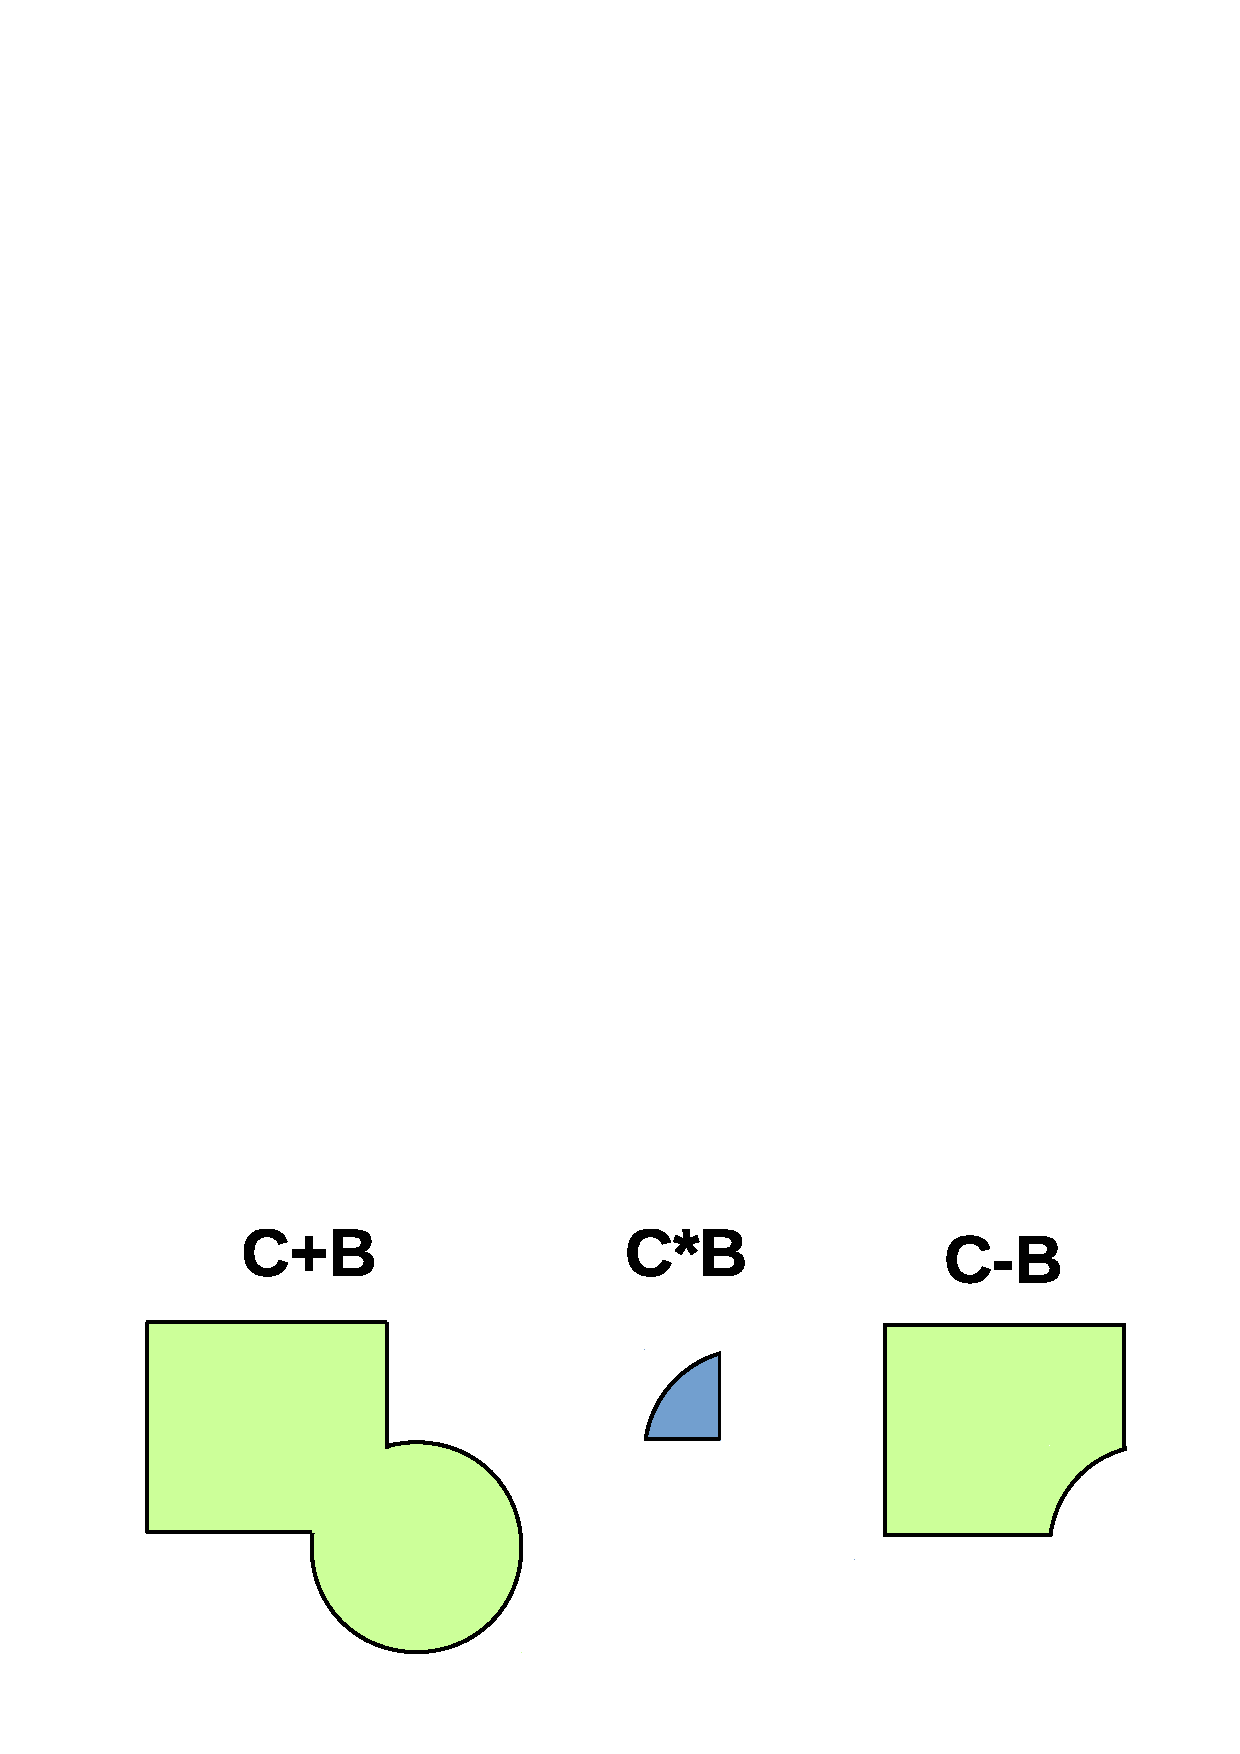
\includegraphics[width=0.6\textwidth]{pictures/Boolean.png}
\caption{Булевы операции.}
\label{fig:Boolean}
\end{figure}

Булевы операции не изменяют уравнений повехностей границ примитивов, а лишь могут сгенерировать новые рёбра на пересечениях граней примитивов. За счёт этого Булевы операции позволяют задать практически любую геометрическую форму, имеющую границы из тех, что применяются в примитивах.

% ================================================================================================================
%  ____       _                               _                                     _              
% |  _ \ ___ | |_   _  __ _  ___  _ __   __ _| |     __ _  ___  ___  _ __ ___   ___| |_ _ __ _   _ 
% | |_) / _ \| | | | |/ _` |/ _ \| '_ \ / _` | |    / _` |/ _ \/ _ \| '_ ` _ \ / _ \ __| '__| | | |
% |  __/ (_) | | |_| | (_| | (_) | | | | (_| | |   | (_| |  __/ (_) | | | | | |  __/ |_| |  | |_| |
% |_|   \___/|_|\__, |\__, |\___/|_| |_|\__,_|_|    \__, |\___|\___/|_| |_| |_|\___|\__|_|   \__, |
%               |___/ |___/                         |___/                                    |___/ 
% ================================================================================================================

\subsection{Полигональное геометрическое представление}\label{sec:secGeoPoly}

% в общем случае - запятые?
Полигональное (тесселированное, фасеточное) представление не менее распростанено, но имеет совершенно другую область применения. Строительным элементом полигональных моделей, в общем случае, является плоский многоугольник, называемый полигоном (polygon, pgon) или фасеткой (facet). Несколько таких многоугольников может стыковаться по рёбрам или вершинам, образуя поверхность, возможно описывающую границы некоторого объекта. Из этого следует, что, строго говоря, полигональное представление является частным случаем BREP с некоторыми допущениями, однако принято рассматривать его как отдельный способ по нескольким причинам.

% Слишком длинное предложение. Надо бы разбить.
В отличии от моделей, предназначенных для таких приложений как моделирование прохождения частиц через вещество или моделирование с помощью МКЭ (например, задач напряжённо-деформированного состояния), где для каждого тела обязательно должны быть определены его границы, отделяющие материал этого тела от окружающего пространства, объект полигональной модели в общем случае не обязан быть замкнутым. Это означает, что, в принципе, между полигонами могут быть зазоры. Это объясняется тем, что полигональные модели изначально рассчитаны на быструю визуализацию, а не выполнение над ними каких-либо расчётов.

Полигональная геометрия в основном применяется в мультипликации, для получения фотореалистичных изображений. При этом основное внимание уделяется не математически точному описанию границ поверхностей, а реалистичности или художественности визуализации модели на дисплее.
%В общем случае такая модель не требует наличия замкнутой оболочки для задания тела, допускается даже остсутствие части границ, если это не влияет на изображение на экране.
Для создания и удобного редактирования полигональных моделей применяется соответствующее ПО: Autodesk 3ds Max, Autodesk Maya, Blender и др.

Частный случай полигонального представления --- триангулированное представление --- имеет треугольники в качестве полигонов. Оно представляет особый интерес т.к. всегда строится для визуализизации на дисплее графической подсистемой того или иного пакета моделирования, даже если пользователь создаёт BREP или CSG. Главная причина для этого заключается в том, что триангулированные модели могут очень быстро обрабатываться 3D-конвейером графического адаптера ПК, как наиболее важный частный случай --- визуализироваться на дисплее.

% http://elanina.narod.ru/lanina/ind/graph/file103.htm

Большинство приложений трёхмерной графики, в том числе САПР, при построении объёмных сцен придерживаются определенной последо­вательности действий, в совокупности составляющей так называемый ЗD-конвейер. В качестве входных данных 3D-конвейер принимает массив треугольников, а итогом работы ЗD-конвейера является отрисовка (рендеринг) резуль­тирующего изображения на дисплее компьютера. Графический адаптер реализует аппаратное ускорение 3D-конвейера.

Несмотря на то что графический адаптер оптимизирован для обработки треугольников, существует ограничение на размер модели, определяемой доступной памятью (как ЦПУ, так и ГПУ). Также объём геометрической модели определяет время её обработки, например, выполнения матричных преобразований при изменении ракурса камеры. Это определяет частоту обновления изображения на дисплее, падение которой ниже некоторого уровня (\todo скажем, 20) сильно усложняет работу.
%Аналогично, увеличение количества элементов в КЭ-модели приводит к увеличению времени расчётов МКЭ.

%OpenGL (Open Graphics Library) --- спецификация, определяющая платформонезависимый (независимый от языка программирования) программный интерфейс для написания приложений, использующих двумерную и трёхмерную компьютерную графику. OpenGL де-факто является стандартом для всех трёхмерных приложений, его конвейер представлен на~\figref{fig:OGLpipeline}.

%\begin{figure}[H]
%\includegraphics[width=0.8\textwidth]{pictures/pipeline-v4.png}
%\caption{Упрощённый конвейер OpenGL. На вход поступают координаты вершин и тройки индексов вершин, образующие треугольник. Выходной результат --- растровое (пиксельное) изображение, пригодное для отображения на дисплее.}
%\label{fig:OGLpipeline}
%\end{figure}

В промышленном геометрическом моделировании триангулированная геометрия применяется не только для визуализации. Например в стереолитографии, и вообще прототипировании, получил распространение формат обмена триангулированной геометрией STL, представляющий собой текстовый файл, в котором перечислены треугольники как группы по три вершины, а вершина задаётся тройкой координат (см. секцию~\ref{sec:secGeoFormats}).

% ================================================================================================================
%  _____ _____ __  __                                     _              
% |  ___| ____|  \/  |     __ _  ___  ___  _ __ ___   ___| |_ _ __ _   _ 
% | |_  |  _| | |\/| |    / _` |/ _ \/ _ \| '_ ` _ \ / _ \ __| '__| | | |
% |  _| | |___| |  | |   | (_| |  __/ (_) | | | | | |  __/ |_| |  | |_| |
% |_|   |_____|_|  |_|    \__, |\___|\___/|_| |_| |_|\___|\__|_|   \__, |
%                         |___/                                    |___/ 
% ================================================================================================================

\subsection{Конечно-элементное (КЭ) геометрическое представление}\label{sec:secGeoFEM}

В инженерной практике широкое распространение получил метод конечных элементов (МКЭ) --- численный метод решения дифференциальных уравнений с частными производными, а также интегральных уравнений, возникающих при решении задач прикладной физики. Метод широко используется для решения задач механики деформируемого твёрдого тела, динамики жидкостей и газов, теплообмена, электродинамики и т.д. МКЭ, как и некоторые другие численные методы, требует геометрическую модель в качестве входных данных.

Метод конечных элементов получил своё название от способа разбиения расчётной области на элементарные блоки --- конечные элементы (КЭ). Строго говоря, КЭ --- это не только геометрическая форма, но и модель аппроксимации решения внутри области, ограниченной этой формой. Существует огромное множество типов КЭ, причём существуют элементы имеющие одинаковую геометрию, но разные математические модели. Расчётная область может быть разбита на элементы различных типов. Исходя из условий решаемой задачи инженер-расчётчик выбирает, какими элементами разбивать расчётную область, а также, обычно, задаёт какие-либо указания модулю разбиения геометрии на сетку в расчётном программном обеспечении. В простом случае расчётной областью является пространство заполненное материалом, т.е. сама деталь, а конечным элементом --- тетраэдр. Модель, в которой деталь представлена множеством КЭ, соответственно называют КЭ-моделью.
% Вырезан кусок... Ушёл в обмен геометриями
